\documentclass[conference,a4paper]{IEEEtran}
\usepackage[T1]{fontenc}
\usepackage{amsmath}
\usepackage{graphicx}
\usepackage{booktabs}
\usepackage{cite}
\usepackage[hidelinks]{hyperref}
\usepackage{xurl}
% generated by code/make_macros.py -- do not edit
\makeatletter
\expandafter\def\csname res@belowNull\endcsname{5}
\expandafter\def\csname res@exAMed\endcsname{$-$1.04}
\expandafter\def\csname res@exANeg\endcsname{36}
\expandafter\def\csname res@exFMed\endcsname{0.90}
\expandafter\def\csname res@exFP\endcsname{<0.001}
\expandafter\def\csname res@exFPos\endcsname{35}
\expandafter\def\csname res@exclHOneNeg\endcsname{30}
\expandafter\def\csname res@exclHTwoNeg\endcsname{16}
\expandafter\def\csname res@exclN\endcsname{41}
\expandafter\def\csname res@hFourHolm\endcsname{=1.00}
\expandafter\def\csname res@hFourN\endcsname{43}
\expandafter\def\csname res@hFourNeg\endcsname{21}
\expandafter\def\csname res@hFourP\endcsname{=1.00}
\expandafter\def\csname res@hFourPos\endcsname{22}
\expandafter\def\csname res@hOneHolm\endcsname{=0.004}
\expandafter\def\csname res@hOneN\endcsname{43}
\expandafter\def\csname res@hOneNeg\endcsname{32}
\expandafter\def\csname res@hOneP\endcsname{<0.001}
\expandafter\def\csname res@hOnePos\endcsname{11}
\expandafter\def\csname res@hThreeHolm\endcsname{=0.02}
\expandafter\def\csname res@hThreeN\endcsname{43}
\expandafter\def\csname res@hThreeNeg\endcsname{30}
\expandafter\def\csname res@hThreeP\endcsname{=0.007}
\expandafter\def\csname res@hThreePos\endcsname{13}
\expandafter\def\csname res@hTwoHolm\endcsname{=1.00}
\expandafter\def\csname res@hTwoN\endcsname{43}
\expandafter\def\csname res@hTwoNeg\endcsname{18}
\expandafter\def\csname res@hTwoP\endcsname{=0.89}
\expandafter\def\csname res@hTwoPos\endcsname{25}
\expandafter\def\csname res@heatMed\endcsname{$-$0.90}
\expandafter\def\csname res@hotThrMax\endcsname{46.1}
\expandafter\def\csname res@hotThrMed\endcsname{35.6}
\expandafter\def\csname res@hotThrMin\endcsname{30.6}
\expandafter\def\csname res@levelBas\endcsname{FPC and PSEI}
\expandafter\def\csname res@levelMax\endcsname{38}
\expandafter\def\csname res@levelMin\endcsname{23}
\expandafter\def\csname res@mapeMed\endcsname{4.23}
\expandafter\def\csname res@medBiasA\endcsname{$-$1.44}
\expandafter\def\csname res@medBiasAll\endcsname{$-$0.08}
\expandafter\def\csname res@medBiasF\endcsname{0.28}
\expandafter\def\csname res@medDays\endcsname{3877}
\expandafter\def\csname res@medNullA\endcsname{$-$2.70}
\expandafter\def\csname res@medNullF\endcsname{$-$0.10}
\expandafter\def\csname res@mzAbove\endcsname{9}
\expandafter\def\csname res@mzAboveSig\endcsname{6}
\expandafter\def\csname res@mzBelowSig\endcsname{28}
\expandafter\def\csname res@mzMed\endcsname{0.96}
\expandafter\def\csname res@nDaysK\endcsname{164}
\expandafter\def\csname res@nEligible\endcsname{53}
\expandafter\def\csname res@nHotMed\endcsname{73}
\expandafter\def\csname res@nLevel\endcsname{2}
\expandafter\def\csname res@nPrimary\endcsname{43}
\expandafter\def\csname res@nRunOne\endcsname{1724}
\expandafter\def\csname res@nRunThree\endcsname{770}
\expandafter\def\csname res@nRunTwo\endcsname{791}
\expandafter\def\csname res@otherMed\endcsname{$-$0.14}
\expandafter\def\csname res@poolA\endcsname{$-$3.01}
\expandafter\def\csname res@poolAHi\endcsname{$-$1.78}
\expandafter\def\csname res@poolAI\endcsname{99}
\expandafter\def\csname res@poolALo\endcsname{$-$4.24}
\expandafter\def\csname res@poolF\endcsname{$-$0.27}
\expandafter\def\csname res@poolFHi\endcsname{0.96}
\expandafter\def\csname res@poolFI\endcsname{99}
\expandafter\def\csname res@poolFLo\endcsname{$-$1.50}
\expandafter\def\csname res@poolHeat\endcsname{$-$0.57}
\expandafter\def\csname res@poolHeatHi\endcsname{$-$0.22}
\expandafter\def\csname res@poolHeatI\endcsname{82}
\expandafter\def\csname res@poolHeatLo\endcsname{$-$0.92}
\expandafter\def\csname res@poolTrend\endcsname{$-$0.09}
\expandafter\def\csname res@poolTrendHi\endcsname{0.37}
\expandafter\def\csname res@poolTrendI\endcsname{98}
\expandafter\def\csname res@poolTrendLo\endcsname{$-$0.55}
\expandafter\def\csname res@robPeakhourOneN\endcsname{43}
\expandafter\def\csname res@robPeakhourOneNeg\endcsname{36}
\expandafter\def\csname res@robPeakhourOneP\endcsname{<0.001}
\expandafter\def\csname res@robRegionOneN\endcsname{13}
\expandafter\def\csname res@robRegionOneNeg\endcsname{9}
\expandafter\def\csname res@robRegionOneP\endcsname{=0.13}
\expandafter\def\csname res@robSecondaryOneN\endcsname{53}
\expandafter\def\csname res@robSecondaryOneNeg\endcsname{41}
\expandafter\def\csname res@robSecondaryOneP\endcsname{<0.001}
\expandafter\def\csname res@robTop10OneN\endcsname{43}
\expandafter\def\csname res@robTop10OneNeg\endcsname{31}
\expandafter\def\csname res@robTop10OneP\endcsname{=0.003}
\expandafter\def\csname res@runOne\endcsname{$-$1.08}
\expandafter\def\csname res@runOneNeg\endcsname{31}
\expandafter\def\csname res@runThree\endcsname{0.44}
\expandafter\def\csname res@runThreePos\endcsname{24}
\expandafter\def\csname res@runTwo\endcsname{$-$0.26}
\expandafter\def\csname res@shareLowMed\endcsname{57}
\expandafter\def\csname res@shareLowPooled\endcsname{60}
\expandafter\def\csname res@trendMed\endcsname{0.00}
\makeatother
\newcommand{\res}[1]{\ifcsname res@#1\endcsname\csname res@#1\endcsname\else\textbf{??#1??}\fi}

\newcommand{\repoURL}{https://github.com/Thanh-Van-2001/ba-peak-forecasts}

\begin{document}

\title{Do Grid Operators Under-Forecast Peak Load? Selection, Heat and a Decade of Day-Ahead Forecasts in U.S. Balancing Authorities}

\author{\IEEEauthorblockN{Thanh Van Nguyen}
\IEEEauthorblockA{Tsinghua Shenzhen International Graduate School, Tsinghua University, Shenzhen, China\\
felicenguyen2001@gmail.com}}

\maketitle

\begin{abstract}
A public scorecard reports that the day-ahead load forecasts of U.S. balancing authorities (BAs) are below demand at the daily peak hour on about 60\% of days. Evaluating forecasts at times chosen by the outcome makes even calibrated forecasts look low (the forecaster's dilemma). Published evaluations of operators' forecasts do not, to our knowledge, separate peak bias from this selection. Using a pre-specified plan and EIA-930 data for \res{nPrimary} BAs (\res{nDaysK} thousand BA-days, 2016--2026), we compare the median error of the daily peak on the 5\% of days with the highest actual peak and on the 5\% with the highest forecast peak. On actual-peak days the forecast was low in \res{hOneNeg} of \res{hOneN} BAs (Holm $p\res{hOneHolm}$); on forecast-peak days in only \res{hTwoNeg} ($p\res{hTwoP}$). By the daily maximum rather than at the peak hour, the forecast was low on \res{shareNegPooled}\% of BA-days. In exploratory analyses, forecasts on forecast-peak days exceeded each BA's usual bias in \res{relFPos} of \res{hTwoN} BAs. We find no evidence of a systematic under-forecast of peak days; the scorecard figure reflects selection. On days above the 95th percentile of summer temperature, the forecast was lower than on other summer days in \res{hThreeNeg} of \res{hThreeN} BAs (Holm $p\res{hThreeHolm}$; pooled \res{poolHeat} percentage points), a shortfall that exploratory analyses place on the first day of a hot spell. Summer-day accuracy did not change between 2016--2019 and 2023--2026. Scorecards should condition on the forecast, and operators should watch the onset of heat.
\end{abstract}

\begin{IEEEkeywords}
Load forecasting, peak demand, forecast evaluation, heat waves, EIA-930.
\end{IEEEkeywords}

\section{Introduction}

A balancing authority (BA) commits generation and schedules reserves a day ahead on the basis of its own load forecast. The forecast of the daily peak matters most. An under-forecast peak leaves the system short of committed capacity on the days it is most stressed, and those days are increasingly hot days \cite{auffhammer2017climate}. Since 2015 every BA in the U.S. Lower 48 has published its day-ahead forecast next to its actual demand on Form EIA-930 \cite{eia930}. This makes it possible to check the forecasts across the country.

Three strands of work bear on whether these forecasts are biased at peaks. The first builds forecasting models. Peak demand research has focused on long-horizon peak densities \cite{hyndman2010density} and on the weather inputs of short-term models: station selection \cite{hong2015weather}, temperature forecast uncertainty \cite{douglas1998impacts}, temperature scenarios \cite{xie2018temperature} and anomalies in temperature data \cite{sobhani2020temperature}; see \cite{hong2016probabilistic} for a review. A recent study finds that models trained mostly on ordinary weather degrade in heat and cold waves \cite{lu2026heat}. These studies test models on historical data, not the forecasts that operators issued. The second strand evaluates the operators' published forecasts. Kazmi and Tao analysed five years of transmission system operators' load, wind and solar forecasts for 16 European countries, comparing accuracy across operators and over time \cite{kazmi2022tso}. For U.S. BAs, the only systematic evaluation we found is a public scorecard, not peer reviewed \cite{cardinalgrid2026,guerrafilho2026note}. It reports that the forecast is below actual demand at the hour of the actual daily peak on about 60\% of BA-days. The third strand, forecast verification, explains why that figure need not indicate a bias.

The natural reading of the figure is that operators systematically under-forecast peaks. That reading is not safe. When forecasts are evaluated at times selected because the outcome was extreme, even a calibrated forecast looks too low. If $E[D\mid F]=F$, days with a high actual load $D$ are disproportionately days on which $D$ turned out above $F$. Lerch et al.\ call this the forecaster's dilemma: outcome-conditioned evaluation rewards forecasters who always predict extremes \cite{lerch2017dilemma}. The clean test of peak bias conditions on the forecast instead. This is the calibration--refinement factorisation of forecast verification \cite{murphy1987framework}, and the logic of calibration and of the Mincer--Zarnowitz regression \cite{gneiting2011point,mincer1969evaluation,murphy1993good}.

\emph{Research gap.} The strands have not met. The evaluations of operators' forecasts report accuracy \cite{kazmi2022tso} or the error at the realised peak \cite{cardinalgrid2026}; to our knowledge, neither separates a peak bias from selection. We found no study that applies the verification tools that can \cite{murphy1987framework,lerch2017dilemma} to operators' load forecasts. The heat studies \cite{douglas1998impacts,lu2026heat} evaluate models, not the forecasts operators used. Whether U.S. operators under-forecast peaks, and whether a shortfall remains in heat, is therefore open. The answer matters for the capacity committed on stressed days and for how scorecards rank operators. The statistical tools we use are standard; the contribution lies in applying them to the forecasts that U.S. operators actually issued, under a pre-registered plan.

We study \res{nPrimary} BAs over 2016 to 2026. The analysis plan was committed to version control before any error was computed for this study. The author had computed errors for four of the BAs in an earlier study of coincident peaks; the plan discloses this. The study asks four questions: do forecasts look low on the days with the highest actual peaks (the scorecard finding); are they low on the days with the highest forecast peaks (the genuine bias); are they lower in heat; and has accuracy changed over the decade? The contributions are:
\begin{enumerate}
\item \emph{A forecast-conditioned test of peak bias in operators' forecasts.} Conditioning on the outcome reproduces the shortfall (forecast low in \res{hOneNeg} of \res{hOneN} BAs); conditioning on the forecast removes it (low in only \res{hTwoNeg} of \res{hTwoN}, $p\res{hTwoP}$).
\item \emph{A decomposition of the scorecard figure into two layers of selection.} Evaluating at the hour of the realised peak raises the share of low forecasts from \res{shareNegPooled}\% to \res{shareLowPooled}\% of BA-days (exploratory). On the days with the highest realised peaks, a calibrated benchmark shows that selection alone can produce the whole shortfall; only \res{belowNull} BAs look lower than their benchmark.
\item \emph{A shortfall in heat, located at its onset.} The forecast is lower on hot days than on other summer days in \res{hThreeNeg} of \res{hThreeN} BAs (Holm $p\res{hThreeHolm}$). By day of hot spell, the median BA's error is \res{runOne}\% on the first day against \res{otherMed}\% on other summer days.
\item \emph{A decade-long check of accuracy}, complementing the European evaluation over time \cite{kazmi2022tso}: summer-day accuracy improved in \res{hFourNeg} BAs and worsened in \res{hFourPos}, with no detectable change.
\end{enumerate}

\section{Data and Methods}

\subsection{Data and sample}
We use the hourly Demand and Demand Forecast columns of the EIA-930 six-month BALANCE files (November 2026 vintage, hashed) for local days 2016-01-01 to 2026-09-30. EIA describes the forecast as the BA's day-ahead forecast. A BA enters the primary sample if its median demand is at least 500~MW and both series are present in at least 80\% of hours in at least 8 of the 11 calendar years. This gives \res{nPrimary} BAs. Dropping the size floor gives \res{nEligible}, the secondary sample. EIA-930 contains recording errors \cite{ruggles2020eia}. Every value that is non-positive, or outside $[0.3, 2]$ times the centred 168-hour rolling median of demand, is set to missing. A day is used only if all its hours have both values. The primary sample has \res{nDaysK} thousand BA-days, a median of \res{medDays} per BA.

\subsection{Peak-day errors and conditioning}
For BA $b$ and day $d$, let $D^*_d$ and $F^*_d$ be the daily maxima of hourly demand and forecast. The peak-magnitude error is $p_d=100\,(F^*_d-D^*_d)/D^*_d$, negative when the forecast is too low. It compares peak magnitudes regardless of the hour. The peak-hour error $e_d$ uses forecast and demand at the hour of $D^*_d$, as the scorecard does. Because the forecast at that hour cannot exceed $F^*_d$, $e_d\le p_d$ on every day.

Even a calibrated hourly forecast has a daily maximum below the expected maximum of demand, so $p_d$ leans negative for every forecast. This works against finding a non-negative bias.

Within each BA and calendar year, which removes load growth, \emph{actual-top} days are those with $D^*_d$ at or above the 95th percentile, and \emph{forecast-top} days those with $F^*_d$ at or above it. We write bias$_A$ and bias$_F$ for the medians of $p_d$ over the two sets.

\subsection{Weather}
For each BA we fixed one to six load-centre cities in the plan, 79 in all. For each city we take the nearest first-order (USW) station of NOAA's GHCN-Daily \cite{menne2012ghcn} with daily maximum temperature on at least 95\% of days. All chosen stations are within 21~km of their city. A BA's temperature is the mean over its cities. A \emph{hot day} is a June to September day at or above the BA's 95th percentile of June to September temperature. The median threshold is \res{hotThrMed}$^\circ$C. Because temperatures are recorded in coarse steps, ties at the threshold give \res{nHotMin} to \res{nHotMax} hot days per BA, with a median of \res{nHotMed}.

\subsection{Hypotheses and tests}
The plan fixed four hypotheses. The unit of inference is the BA.
\begin{itemize}
\item H1: bias$_A<0$ in a majority of BAs.
\item H2: bias$_F<0$ in a majority of BAs.
\item H3: within June to September, median $p_d$ on hot days minus that on other days is negative in a majority of BAs.
\item H4: median $|p_d|$ over June to September days in 2023--2026 minus that in 2016--2019 differs from zero in sign more often than chance.
\end{itemize}
H1 to H3 use one-sided and H4 two-sided binomial sign tests, with Holm's adjustment over the four \cite{holm1979simple}. H2 tests against zero as pre-specified; a sharper test of a peak-specific bias compares bias$_F$ with each BA's overall bias (exploratory, below).

Five secondary analyses were pre-specified:
\begin{enumerate}
\item \emph{Pooled effects:} DerSimonian--Laird random-effects means \cite{dersimonian1986meta}, with BA-level standard errors from a moving-block bootstrap \cite{kunsch1989jackknife} with 7-day blocks and 2{,}000 replicates.
\item \emph{A calibrated benchmark:} within each BA-year we shuffle the ratios $D^*_d/F^*_d$ across days 200 times, keeping $F^*_d$ fixed. This makes the forecast calibrated up to its mean bias. Recomputing bias$_A$ then shows how low a forecast looks on actual-top days through selection alone.
\item \emph{The Mincer--Zarnowitz slope} of $D^*_d$ on $F^*_d$ over summer days, with Newey--West intervals \cite{newey1987simple}. A slope below one means the forecast peaks move too much.
\item \emph{Robustness variants} (Table~\ref{tab:robust}). The regional variant lets each EIA region vote with the majority sign of its BAs.
\item \emph{Errors by day of a hot spell.}
\end{enumerate}
A pipeline check ran on CISO and ERCOT for 2018 before the full run.

\emph{Amendment.} After the results and an internal review, we fixed three bugs: the bootstrap's last block start, hot-spell runs counted on days with valid load instead of on the temperature series, and a regional median used in place of the majority vote. None changed a hypothesis outcome. We also added the exploratory analyses marked below. All are logged as Amendment 1 in the plan.

\section{Results}

\subsection{The scorecard figure and where it comes from}
At the hour of the actual daily peak, the forecast was below demand on \res{shareLowPooled}\% of all BA-days, matching the scorecard \cite{cardinalgrid2026}. Measured by the daily maximum $p_d$, the forecast was low on \res{shareNegPooled}\% of BA-days, and on \res{shareNegMed}\% in the median BA (exploratory). The median BA's overall bias was \res{medBiasAll}\%. Most of the scorecard's excess over one half thus comes from evaluating the forecast at the hour of the realised peak, a within-day form of outcome selection.

\subsection{Actual-peak days versus forecast-peak days}
H1 was supported. On actual-top days, bias$_A$ was negative in \res{hOneNeg} of \res{hOneN} BAs ($p\res{hOneP}$, Holm $p\res{hOneHolm}$). The median was \res{medBiasA}\%.

H2 was not supported. On forecast-top days, bias$_F$ was negative in only \res{hTwoNeg} of \res{hTwoN} BAs ($p\res{hTwoP}$). The median was \res{medBiasF}\%.

Fig.~\ref{fig:bias} shows the pattern BA by BA. In all \res{nFgtA} BAs the forecast-top marker lies to the right of the actual-top marker. Some separation is expected for any noisy forecast. What matters is where the forecast-top marker sits relative to zero, and it sits on both sides.

Two BAs, \res{levelBas}, have a forecast \res{levelMin}--\res{levelMax}\% below demand on all days alike. This level gap suggests that their two series measure different quantities. They dominate the pooled means, which are \res{poolA}\% for bias$_A$ and \res{poolF}\% for bias$_F$. Without them (exploratory), the pooled bias$_A$ is \res{poolAEx}\% (95\% CI \res{poolAExLo} to \res{poolAExHi}) and the pooled bias$_F$ is \res{poolFEx}\% (CI \res{poolFExLo} to \res{poolFExHi}).

The conclusion survives every variant in Table~\ref{tab:robust}, with one weakening. When each EIA region casts one vote, H1 is no longer significant (\res{robRegionOneNeg} of \res{robRegionOneN} regions, $p\res{robRegionOneP}$), because neighbouring BAs share weather. Two notes on the table:
\begin{itemize}
\item Using the second-highest hour of each day, so that a single-hour forecast spike cannot select a day, gives the same counts (exploratory).
\item With EIA's adjusted demand the counts equal the primary ones, although the BA-level values are identical in only \res{adjEqual} BAs.
\end{itemize}

\begin{figure}[t]
\centering
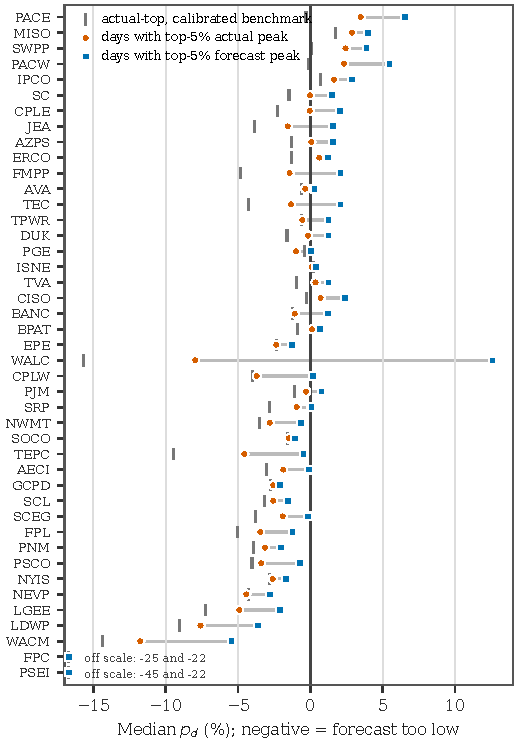
\includegraphics[width=\columnwidth]{fig_bias.pdf}
\caption{Median peak-magnitude error $p_d$ over each BA's actual-top days (circles) and forecast-top days (squares), the days being chosen within each calendar year. Ticks: the same statistic for a calibrated forecast with the BA's own errors (shuffle benchmark). BAs sorted by their bias over all days. Two BAs are off scale.}
\label{fig:bias}
\end{figure}

\begin{table}[t]
\caption{Sign tests under the pre-specified variants: BAs (or regions) with negative bias, and one-sided $p$. $^\dagger$Exploratory (Amendment 1).}
\label{tab:robust}
\centering
\begin{tabular}{lrrrr}
\toprule
 & \multicolumn{2}{c}{H1: actual-top} & \multicolumn{2}{c}{H2: forecast-top} \\
\cmidrule(lr){2-3}\cmidrule(lr){4-5}
Variant & neg. & $p$ & neg. & $p$ \\
\midrule
\csname @@input\endcsname tab_robust.tex
\bottomrule
\end{tabular}
\end{table}

\subsection{Selection explains the shortfall on actual-peak days}
In the calibrated benchmark, selection alone would make the median BA look \res{medNullA}\% low on actual-top days. The observed value is \res{medBiasA}\%, and only \res{belowNull} BAs look lower than their benchmark. With the shuffle restricted to calendar months, so that the benchmark respects season, no BA looks lower (\res{belowNullMonth} of \res{hOneN}; exploratory). Selection is thus large enough to account for the whole shortfall.

The benchmark treats errors as exchangeable within a month. If percentage errors are smaller on high-load days, it overstates selection. So the comparison does not by itself show that operators over-forecast.

Two further diagnostics point the same way:
\begin{itemize}
\item \emph{The Mincer--Zarnowitz slope} had a median of \res{mzMed}. It was significantly below one in \res{mzBelowSig} BAs and above one in \res{mzAboveSig}. With year fixed effects and a robust fit (exploratory), the counts are \res{mzrBelowSig} and \res{mzrAboveSig}. When an operator forecasts a high peak, the actual peak tends to fall short of it.
\item \emph{Relative to each BA's overall bias} (exploratory), the forecast on forecast-top days was higher in \res{relFPos} of \res{hTwoN} BAs ($p\res{relFP}$; median \res{exFMed} percentage points). On actual-top days it was lower in \res{relANeg}.
\end{itemize}
Leaning high on expected peak days is what an optimal forecast does when shortfalls cost more than surpluses \cite{patton2007optimal}. Our data cannot say whether it is deliberate.

\subsection{Heat}
H3 was supported. On hot days the median error was lower than on other summer days in \res{hThreeNeg} of \res{hThreeN} BAs ($p\res{hThreeP}$, Holm $p\res{hThreeHolm}$). The pooled difference was \res{poolHeat} percentage points (CI \res{poolHeatLo} to \res{poolHeatHi}; Fig.~\ref{fig:heat}a), and \res{poolHeatEx} without the two level-gap BAs.

The pre-specified analysis by day of spell locates the effect (Fig.~\ref{fig:heat}b). The median BA's error was:
\begin{itemize}
\item \res{runOne}\% on the first hot day of a spell;
\item \res{runTwo}\% on the second;
\item \res{runThree}\% from the third day on;
\item \res{otherMed}\% on other summer days.
\end{itemize}
Exploratory tests confirm the pattern:
\begin{itemize}
\item The first day was below other days in \res{runOneOtherNeg} of \res{hThreeN} BAs ($p\res{runOneOtherP}$).
\item Third-or-later days were below other days in only \res{runThreeOtherNeg}.
\item Within spells of at least three days, the first day was below the third-or-later days in \res{spellNeg} of \res{spellN} BAs ($p\res{spellP}$; median \res{spellMed} points).
\item On the day after a hot day, when heat is easier to anticipate, the forecast was lower than on other days in only \res{heatLagNeg} BAs (median \res{heatLagMed}).
\end{itemize}

The shortfall appears when heat arrives, not while it lasts. Hot days are chosen by observed temperature. A day selected as hot is more often one that turned out hotter than forecast, and this is most likely for the first day of a spell. The onset effect is therefore consistent with temperature forecast error \cite{douglas1998impacts} as well as with a lag in the load model, and our data cannot separate the two.

\begin{figure}[t]
\centering
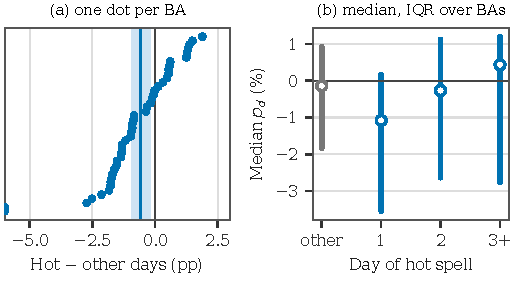
\includegraphics[width=\columnwidth]{fig_heat.pdf}
\caption{(a) Median $p_d$ on hot days minus that on other June--September days, one dot per BA; band: pooled random-effects mean and 95\% CI. Two BAs below $-6$ are drawn at the edge. (b) Median and interquartile range over BAs of the median $p_d$ on other summer days and on the first, second and later days of runs of hot days (\res{nRunOneDays}, \res{nRunTwoDays} and \res{nRunThreeDays} BA-days in all).}
\label{fig:heat}
\end{figure}

\subsection{No change over the decade}
H4 was not supported. The median absolute error over summer days fell in \res{hFourNeg} BAs and rose in \res{hFourPos} ($p\res{hFourP}$). The pooled change was \res{poolTrend} percentage points (CI \res{poolTrendLo} to \res{poolTrendHi}). We cannot detect a change in summer-day accuracy at this resolution.

\section{Discussion}

The public statistic ``the forecast is low at the peak on 60\% of days'' is accurate as a description and misleading as a diagnosis. Two layers of selection build the shortfall in:
\begin{itemize}
\item choosing the hour of the realised peak;
\item choosing the days with the highest realised peaks.
\end{itemize}
Conditioning on the forecast removes the shortfall, and the regression slope even reverses it. This is the forecaster's dilemma \cite{lerch2017dilemma} at work on a national data set. A scorecard that ranked BAs by their error at realised peaks would reward operators who inflate their peak forecasts. We recommend that scorecards report calibration conditional on the forecast, through the bias on forecast-top days or the Mincer--Zarnowitz slope. To rank forecasts they should use proper scores or, for point forecasts, consistent scoring functions, weighted toward the upper tail when peaks matter \cite{gneiting2011comparing,taggart2021point}; unlike scores computed on outcome-selected days, these cannot be improved by inflating forecasts.

Heat is where a shortfall remains, and it is concentrated at the onset of a hot spell. For operators, the lesson is to examine the first day of a heat wave: both the temperature inputs \cite{sobhani2020temperature,douglas1998impacts} and the response of the load model, which can degrade in extremes \cite{lu2026heat}. For capacity and reserve planning, the first hot day is the riskiest day.

\subsection*{Limitations}
\begin{itemize}
\item EIA-930 does not document each BA's forecast issue time or method.
\item One to six stations per BA approximate its weather.
\item Hot days are defined by observed temperature, not by the forecast the operator used.
\item BAs are not independent; the regional test for H1 is not significant.
\item The calibrated benchmark assumes exchangeable errors within a month.
\item The screen removes gross errors only.
\item The peak-hour error $e_d$ is sensitive to timestamp offsets in the forecast series, such as the one-hour shift in PJM's forecast series from 2019 on, also reported in an erratum to the scorecard note \cite{guerrafilho2026note}. The primary measure $p_d$ compares daily maxima and is not affected.
\end{itemize}

\section{Conclusion}
Across \res{nPrimary} U.S. balancing authorities and a decade of data, we find no evidence that operators under-forecast peak days. The widely quoted shortfall reflects evaluation at realised peaks. A real shortfall appears on the first day of heat. Forecast scorecards should condition on the forecast, not on the outcome.

\section*{Data and code availability}
The analysis plan with its commit history and amendment, the code, the station list and the result files are available at \url{\repoURL}. The EIA-930 and GHCN-Daily data are public.

\section*{Acknowledgment}
The author used Claude Opus 5.5 (Anthropic; model identifier claude-opus-5-5) to help write analysis code and draft and edit the text. The author checked the code, the results and the text and takes full responsibility for the content.

\bibliographystyle{IEEEtran}
\bibliography{refs}

\end{document}
